\chapter{Discussion}
This chapter contains various discussion topics, including: validity of my research and of the analytics tools, where the various analytics tools provide the most value, ethics and legal aspects, abandoned apps, and finally other app stores beyond Google Play.
%TBD whether to include a discussion of:
%%% other analytics tools I've researched during my PhD (e.g. those covered in my probation report)
%%% sweetspots for Crashlytics, Firebase, etc.

If we focus on Android apps what are the implications and how relevant are the approaches and results? Apps are a popular and relevant subset of all software,they run remotely on other people’s equipment where they are the primary owners of the data on their devices, and where the platform and pre-installed platform software determine various aspects of the data collection

\section{On Measurement}
Measurement may begin using rough and approximate measurements and tools, for instance the length of a yard which used to depend on the span of the king's arm~\footnote{One source is:~\url{http://nisltd.co.uk/asp/default.aspx?page=history_of_calibration}}. France, in particular, led to the standardisation of various measurements including the metre~\footnote{\emph{e.g.}~\url{http://www2.culture.gouv.fr/culture/actualites/celebrations/metre.htm} (in French).}

Software development and testing are still in flux where various people and groups have yet to coalesce or truly agree to common, unambiguous and definitive measurements. Even newer standards, including~\cite{iso29119-1-2013}, which were intended to provide a pragmatic and useful guide to practitioners (\cite{reid2012_iso29119_eurostar}), would only be used by a minority (19\% according to a poll by EuroSTAR Conferences in 2013~\footnote{\url{https://conference.eurostarsoftwaretesting.com/poll-result-will-you-be-using-iso-29119-standards-in-your-testing/})} of an estimated 60 respondents to the poll~\footnote{\url{https://conference.eurostarsoftwaretesting.com/standards-a-case-for-the-defence/}}.

How to measure anything. 

My research into the \emph{use} of mobile analytics tools led into research into the characteristics of several of the actual tools in widespread use by developers of mobile apps. The measurements and assessments of these tools is immature and my work provides a possible starting point to enable these and other analytics tools to be measured and assessed.

\section{Threats to Validity}
Using ratings and reviews to measure quality? Tim Menzies quote on software analytics. 

\subsection{Validity of my research}

\subsection{Validity of the tools being used?}

\subsection{Quis custodiet ipsos custodes?}
\url{https://en.wikipedia.org/wiki/Quis_custodiet_ipsos_custodes%3F}
Who watches the watchers? The app store is all powerful, promoting one app, demoting or even blocking another. What it reports is expected to be taken on trust. And who has time or resources to check or verify the veracity of what is being reported and to whom? 


\subsection{Necessary? Sufficient?}
Freezes and crashes may adversely impact a user's perspective, Google may limit the visibility of apps that score poorly in terms of 'stability' as I will cover later in my thesis. However, are performant applications sufficient to thrive? There may be other barriers, or hurdles, developers need to overcome such as providing software that is attractive, serves whatever the user wants to do, and is intuitive.

In 2019 Menzies in his paper \emph{``Take Control: On the Unreasonable Effectiveness of Software Analytics"}~\cite{menzies2019take} indicates that a small number of predictable software analytics variables can be used to predict software qualities for projects. 

\emph{``Specifically, the number of variables required to make predictions about SE projects is remarkably small which means that (a) most of the things we think might affect software quality have little impact in practice; (b) controlling just a few key variables can be enough to improve software quality."}

\subsection{External Validity}
I have been fortunate to receive external confirmation from various external sources that the research is of interest and appears to have some validity. These include:

\subsubsection{Validity from the Google Engineering Team}

MUST\_DO Use the beyond Google Play paper to help support the validity of my research.

\subsubsection{Other validation}
In email discussions of my research in 2020 one of the leading authors in the field, \href{https://scholar.google.com/citations?user=zuUsFkgAAAAJ&hl=en&oi=sra}{Li Li}, confirmed the novelty, importance and relevance of my research.



\section{Android Vitals}
\subsection{Which apps can Android Vitals help?}
As Google only provides various reports in Android Vitals once they decide enough data exists to preserve the privacy of end users Android Vitals provides little for developers of less popular apps. 

Based on very rough approximations combining my case studies with AppBrain's download statistics to 19th June 2019, shown in figure \ref{fig:appbrain_download_statistics_jun_2019}\cite{appbrain_download_statistics_june_2019}, of the total populations of app developers:
\begin{itemize}
    \item 3\% to 4\% (those with 100,000 to 500,000 total downloads) will get limited value as at least one report will be provided.
    \item < 1\% (those with 500,000 to 1,000,000 total downloads) will get some value as many of the reports will be provided, but not all.
    \item 1\% (those with > 1,000,000 total downloads) will get extensive value as most/all the reports will be provided.
\end{itemize}

\begin{figure}
    \centering
    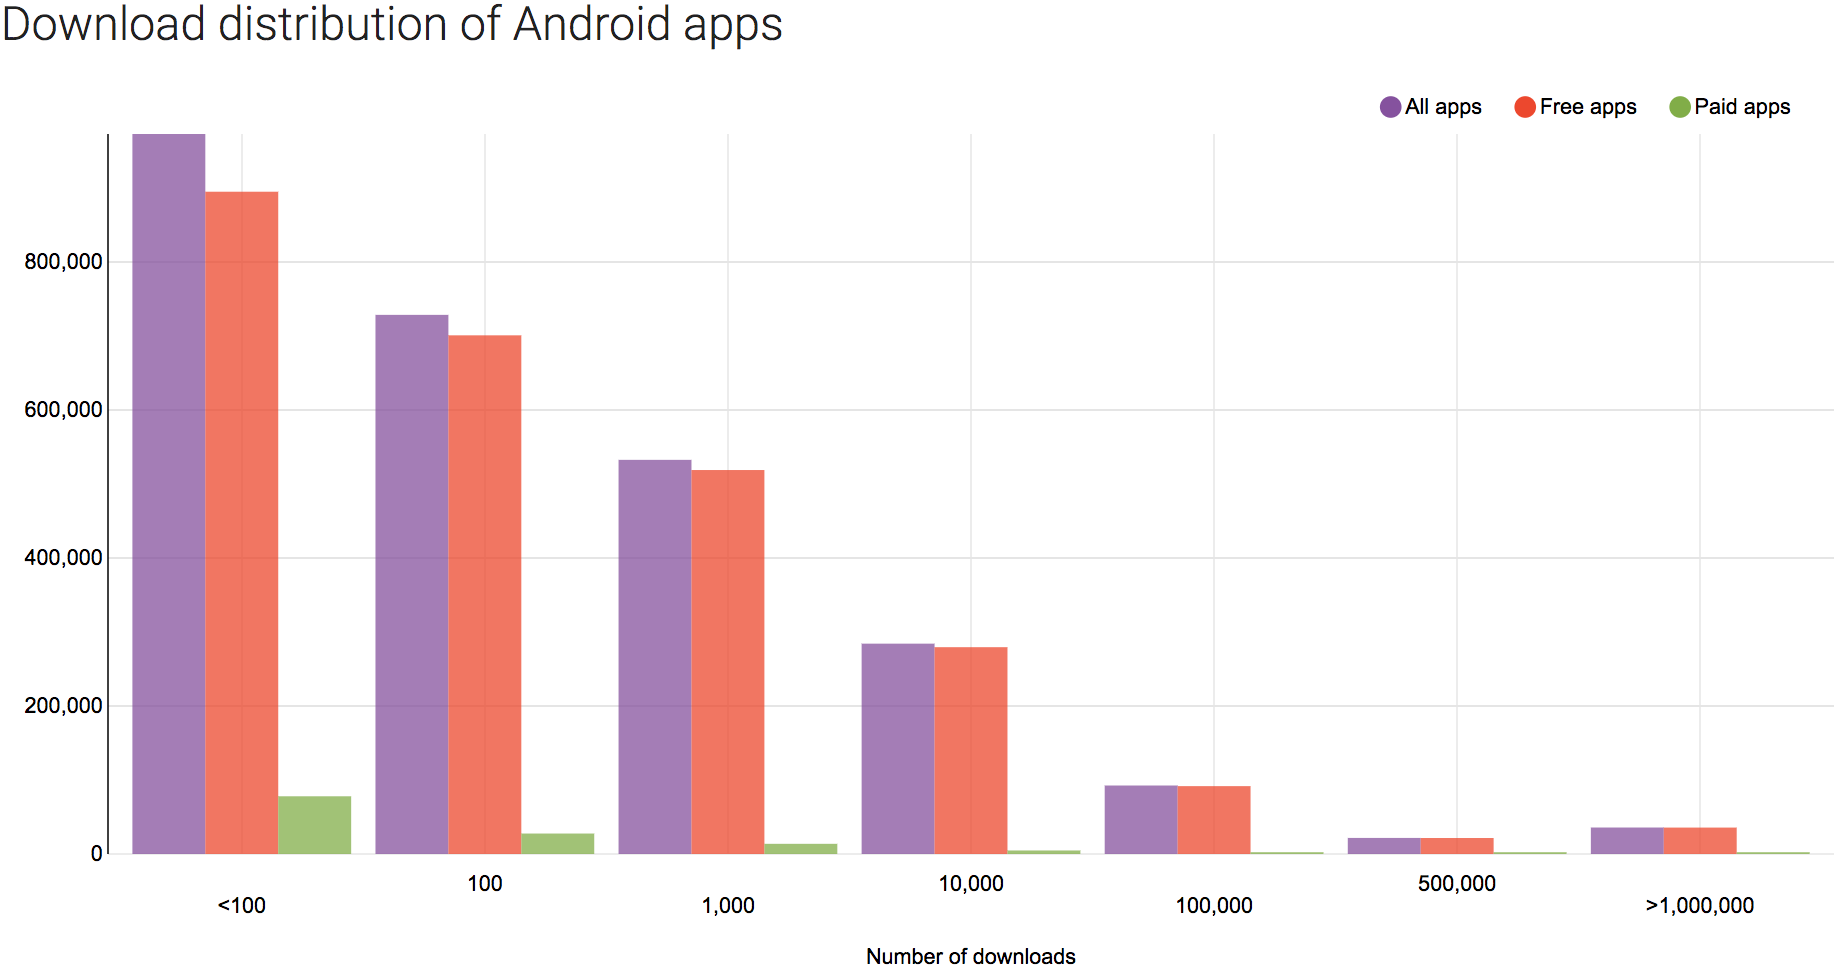
\includegraphics[width=\textwidth, keepaspectratio]{images/appbrain/AppBrain_Download_Statistics_20-Jun-2019.png}
    \caption{AppBrain: Download distribution of Android apps (June 2019)}
    \label{fig:appbrain_download_statistics_jun_2019}
\end{figure}

\subsection{Who gets sufficient usage to see more detailed reports?}
Our limited insight into Android Vitals already indicates that reports are only provided when there is sufficient data collected to 'prime the pump'. It may be possible to estimate how many apps of those in Google Play Store are likely to have enough volumes of usage data. Google makes various recommendations for developers on how to apply the results Android Vitals reports \url{https://developer.android.com/distribute/best-practices/develop/android-vitals} however the developers can't do much until Android Vitals actually shows them the data. For apps with less than about 50k active installs \textit{("Installs on Active Devices (devices online in the past 30 days with this app installed)}." according to Google Play Console's tool tip). These counts are around 20\% to 30\% of the total install count for various apps used in our research \textit{e.g.} the active installs would be around 20k for an app that shows at having 100,000+ [total] installs to end users in Google Play.

Data provided by AppBrain\cite{appbrain_download_statistics_june_2019} was used to estimate the populations of apps that are not likely to generate enough data to see various reports in Android Vitals.
% wikimedes 5373 active installs - Crash rate by app version only (not device or Android version).
% wikimedzh 3769 active installs - no Android Vitals reports
% wikimedfa 2807 active installs - no Android Vitals reports
% 
Based on Android Vitals reports for Kiwix custom apps we infer that few apps with less than 20,000 total installs will have any detailed reports; WikiMed in Spanish has 5,373 active installs and has one report, for crash rate by app version. None of the other reports are available for this app. The threshold for when there is enough data for Google to provide a report depends on various factors, so the total installs is a proxy measurement and imperfect. Therefore Android Vitals is unlikely to offer much value for developers of (973,381 + 730,419 + 553,261 + 284,634) apps i.e. 2,541,695 apps in Google Play. For the next 92,678 the value of Android Vitals might increase somewhat, depending on how their app behaves and their user-base (e.g. are they on a few Android versions or spread across a spectrum - the larger the spread the less likely the reports will have data). And so on. By my admittedly limited view into the overall data set, Android Vitals is best placed to help the developers of the top (21,728 + 35,854) 57,582 apps, approximately 2\% to 3\% of the total population (2,691,955 apps). These apps (according to AppBrain's data on library use) are also more likely to use Firebase, Crashlytics, etc. so also have some of the run-time data available from these sources in addition to Android Vitals.

My work is to investigate two broad sources of data - data collected by the operating system (here effectively what appears in Android Vitals) and data collected using in-app libraries, particularly mobile analytics, it could include heatmapping (e.g. Appsee, found in over 790 Android apps with over 375 million downloads~\cite{appbrain_appsee}), crash handlers, etc. to provide feedback to measure how well the development team did in terms of testing and code quality. What they learn could also be useful to help them improve how they develop and test their apps in future, particularly with the greater detail mobile analytics (particularly Firebase) can provide the team.

\subsection{All that glitters is not gold}
Android Vitals sometimes reports excessive network usage running in the background while the device is running on battery, as shown in figure \ref{fig:android_vitals_excessive_network_usage}. As the Kiwix app is designed to enable users to download sometimes extremely large files, and to do so in the background, this warning is to be expected and not a bug - it's a feature. So, not everything that Android Vitals flags necessarily needs to be acted on. 
\begin{figure}[ht]
    \centering
    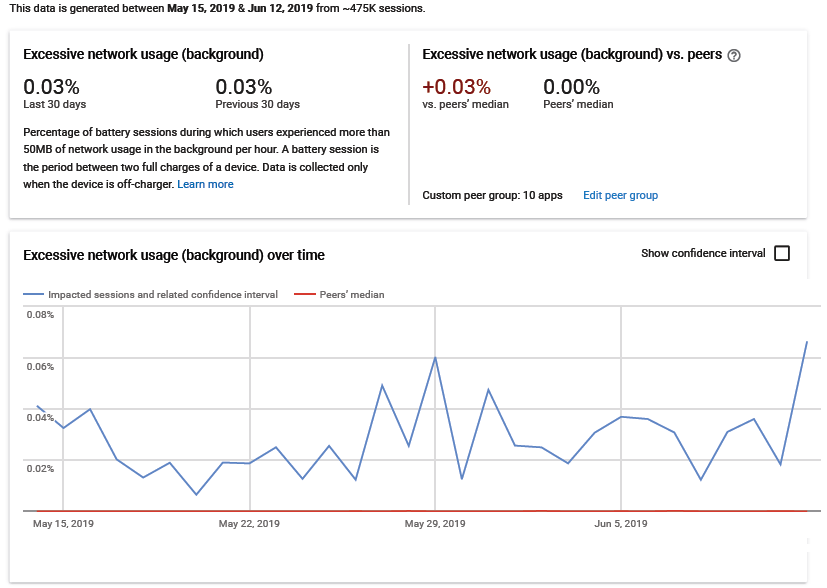
\includegraphics[width=\textwidth, keepaspectratio]{images/android-vitals-screenshots/Excessive_network_usage_by_kiwix_15_jun_2019.png}
    \caption{Excessive background network usage on battery}
    \label{fig:android_vitals_excessive_network_usage}
\end{figure}

\section{Ethics of incorporating mobile analytics}
Tradeoffs; comparing other approaches which may have similar effect with less/no tracking.

\subsection{Litigation on unwanted data collection}
On \nth{14} July 2020, a case was filed in Northern California, USA as a class action against Google and the parent company Alphabet~\cite{rodriguez_et_al_v_google_llc_et_al_2020} stating \emph{``No matter what safeguards are put in place, mobile app users cannot prevent Google intercepting, collecting, tracking and selling for profit their browsing histories and internet activity."} where the plaintiffs investigate the behaviours of Google with a particular emphasis on the use of Firebase Analytics which does not honour Google's claimed commitments to end users to be able to disable such data from being shared by their Android device. Blogs, including~\cite{winder2020_forbes_on_the_class_action_firebase_analytics}, discuss the claims and several related recent incidents pertaining to Firebase.

These incidents include data leakages where developers did not secure their Firebase databases appropriately, as reported in~\cite{bischoff2020_firebase_missconfiguration} the configurations do not appear to be secure by default. Firebase databases are distinct from Firebase Analytics, however one might infer that developers who don't secure their Firebase databases (which are incorporate into their apps by the same development team) they may be similarly insecure in their use of Firebase Analytics. According to a news article by Reuters~\cite{dave2020_reuters_firebase_squeeze} Google are pushing developers to integrate Firebase into their apps through offering improved business benefits for that app's ecosystem. If the claims are accurate then even more developers are likely to use Firebase and Firebase Analytics. Unless those developers actively consider and mitigate for privacy related features that users can control there may be additional ethical concerns.

% https://www.classaction.org/news/always-watching-class-action-against-google-alleges-user-privacy-doesnt-exist#embedded-document
% https://lawstreetmedia.com/tech/google-is-always-watching-class-action-complaint-says/
% https://www.reuters.com/article/us-alphabet-google-privacy-lawsuit/google-faces-lawsuit-over-tracking-in-apps-even-when-users-opted-out-idUSKCN24F2N4
% https://www.scribd.com/document/469160855/2020-07-14-Dkt-1-Rodgriguez-Et-Al-v-Google-LLC-Et-Al#download
% 

\subsection{Beware of implicit, automated data collection}
There are various considerations of the adverse implications of allowing, and using, implicit automated data collection, such as often performed by mobile analytics libraries in industry. A simple example is that the library implementer may choose to change the functionality of the automatic data collection, rename, restructure, or remove content developers have come to expect and rely on, etc. This topic is discussed in a blog post by Iteratively~\cite{mukherjee_implicit_versus_explicit_event_tracking_hits_and_misses}.

A more involved example started in March 2017 where the Mixpanel JavaScript SDK which inadvertently collected passwords and might have collected other highly sensitive data such as \emph{``where browser plugins (such as the 1Password password manager) and website frameworks place sensitive data into form element attributes."}~\cite{mcclintok_mixpanel_update_on_autotrack_data_collection}. 

According to the post, the problem did not exist when they designed and launched the service in 2016, it was triggered when they updated the version of an external and well regarded library in March 2017. The issue was discovered and reported by a customer in January 2018. Mixpanel deleted the sensitive data their library had collected on behalf of their customers and implemented various corrective actions including in-depth security reviews of existing code. They also had to put in place filters to delete new data on arrival as some of their customers were still using the ill-mannered implementation of their JavaScript SDK.

\subsubsection{A related finding in our PocketCode case study}
In February 2020 the Catrobat team migrated the reporting for their app crash analytics (Crashlytics) from the Fabric website to the Firebase website using an inbuilt migration tool provided by Google who own both services. The migration meant the app's crash data could be viewed in both these websites independently until Google disabled the Firebase website (planned for March, but postponed until \nth{4} May 2020 in response to the effects of the COVID-19 pandemic).  We noticed additional data was available and presented in the reports provided in the Firebase console, as Google describe the website. This includes demographic data \emph{even though this is not collected by our app or - officially - by the crashlytics libarry}! Figure \ref{fig:Firebase-event-demographics-pocketcode-android} provides an example of the relevant section of the `Events' report for the Pocket Code Android app. App developers may, understandably, be unaware that using a library for collecting crash data is also somehow gathering data about demographics, therefore their end user licence agreements (EULA), privacy policy, and so on, may not reflect or incorporate this information to inform the user of what is being collected and why (in potential contravention with GDPR and other legislation).

\begin{figure}[ht]
    \centering
    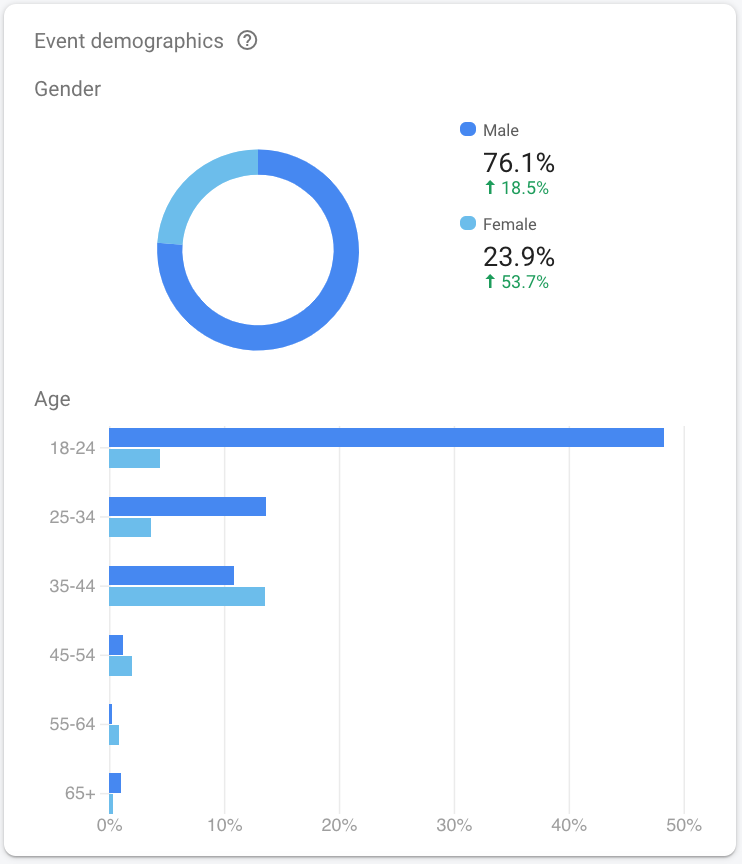
\includegraphics[width=8cm]{images/firebase/Firebase-event-demographics-pocketcode-android.png}
    \caption{Firebase Event Demographics for Pocket Code Android}
    \label{fig:Firebase-event-demographics-pocketcode-android}
\end{figure}

Practical options:
\begin{itemize}
    \item Do as others do?
    \item Proportionate exchange of value: users do not pay for the app, and few actively provide feedback. Organ donation is far more intrusive and yet English law is changing\footnote{\url{https://www.organdonation.nhs.uk/uk-laws/}} to presume consent\cite{NHS_organ_donation_in_england} 
    \item Offer an opt-out
    \item Offer an opt-in
    \item leave the user to take action to provide information c.f. Kiwix-Android and Android Daisy Reader.
\end{itemize}

\subsection{Legal aspects of using mobile analytics for development and testing}

\begin{itemize}
    \item GDPR?
    \item PII vs non-PII information.
\end{itemize}

Data ownership and safeguarding.

\subsection{Considerations and concerns when using Mobile Analytics}
\begin{itemize}
    \item Privacy:
    \item Costs: financial, data, privacy, performance, bloat:
    \item Who owns the data and who gets to use it?:
    \item Stewardship: Impact(s) of having access to sensitive and valuable data.
    \item Performance:
    \item Sufficiency: is the data we collect sufficient to enable us to achieve our objectives of improving testing.
    \item [Over] trust in decisions made by technology.
\end{itemize}

\subsubsection{Human behaviours around automation}
The use of software automation can have deep implications on the humans involved, ranging from emotional stress and worries where testers on development teams can get stuck where tools are expected to solve problems (but don't)~\cite{evans2020stuck}, to potentially over-reliance on the decisions made by automation~\cite{cummings2004automation} and a complacency and bias in human interaction with automated and decision support systems~\cite{parasuraman_complacency_and_bias_in_human_use_of_automation}. 
My experiences of email discussions with the Google Engineering team provided an impression they over-believed in the correctness of their analytics tools and the inability of any outsider being able to understand their system. This is somewhat ironic given that I was a senior software quality engineer at Google for four years and worked on assessing the behaviours and qualities of Google's mobile apps for several years during that role.

\section{Additional considerations}
This section covers several additional topics, including: abandoned apps, additional app stores beyond Google Play and beyond Android, and implications for apps stores for medical devices?

\subsection{Abandoned Apps}
Users are not the only people who many abandon apps, developers do so too. By the very nature of abandoning an app a developer is also likely to abandon the reports and data associated with that app, including data from mobile analytics. As many researchers discover there are many abandoned opensource source code repositories, and similarly various organisations, including AppBrain, have identified apps that are effectively abandoned. % MUST-DO add citation for AppBrain report.

\subsection{The Reaper Cometh}
AppBrain is a business that actively monitors and reports on Android Apps in the Google Play Store. The business was founded by two ex-Google engineers, as I am. They state Google is actively culling Android apps from the Google Play store and estimate approximately 16\% of apps are \emph{"low quality apps"} and \emph{"unlikely to be useful"}~\footnote{\url{https://www.appbrain.com/stats/number-of-android-apps}} % Percentage of low quality apps: 16%


\subsection{Other Android App Stores?}
Note: this research is limited to apps available in Google Play for practical reasons. Other Android app stores are available, particularly in China as Wang ~\emph{et al} (2018)~\cite{wang2018beyond} describes. Of the Chinese app stores, in 2018 only 2 (Tencent Myapp, and 360 Market) provided a quality rating. 

\subsection{Applicability to Other App Stores?}
App Stores were popularised for mobile apps for Android, iOS, and other smartphone platforms now extinct (\emph{e.g.} Windows Mobile), even if App Stores existed several years before smartphones did. % COULD_DO cite early versions of the Mobile Developer's Guide to the Galaxy, etc.

They then spread to other mainstream operating systems including OSX, some Linux distributions, etc. using a similar business and software development model to the Android and iOS app stores. Recently, e.g. in 2019, App Stores were also reported for Radiology - for instance in an article in Harvard Business Review on \emph{What AI ``App Stores" will mean for Radiology}~\cite{hbr_what_ai_app_stores_mean_for_radiology}. The authors of the article envisage various benefits that emerge from applying a \emph{marketplace model} for these apps, including better feedback for developers. In tandem, the importance of incorporating appropriate analytics and ensuring they are trustworthy also seems worthy of further research and analysis. 

\section{Summary of the Discussion Chapter}
My research indicates mobile analytics can be used to effectively and efficiently improve the measured stability qualities of various Android apps from disparate sources, development teams and software stacks. And yet, there are appear to be material flaws in key analytics tools. My research touches on various implications of using analytics including which projects are best served by the integral analytics Google provides in Google Play Console. There are numerous areas of potential interest to researchers and industry alike including the integrity and accuracy of the various tools and reports. I will introduce my planned future work in the Future Work chapter.